\documentclass[12pt,a4paper]{article}
\usepackage{graphicx}
\usepackage[french]{babel}
\usepackage{hyperref}
\usepackage{caption}
\usepackage{subcaption}
\usepackage{float}
\begin{document}
	\begin{titlepage}
		\newcommand{\HRule}{\rule{\linewidth}{0.5mm}}
		\center
		\textsc{\large
			Département de Mathémathiques et Informatique \\[0.25cm]
			Faculté des Sciences Exactes et Appliquées \\[0.25cm]
			Université de N'Djamèna \\[0.25cm]
			\centering \textbf{---}\\[0.25cm]
			Simplonline.co \\[0.25cm] Tech4Tchad 
		} \\[1.5cm]
		%\includegraphics[scale=0.5]{logo.png} \\[1cm]
		\HRule \\[0.15cm]
		{ %\huge
			\bfseries Machine Learning \\ t-SNE : t-distributed Stochastic Neighor Embedding \\[0.15cm] }
		\HRule \\[1.5cm]
		HAMIDE Mahamat \\
		HASSANE MOUSTAPHA Ousmane \\
		Honoré PAYANG \\
		MAHAMAT NIL Hassan \\
		MBA LE IRAN Ezechiel
		\\[1.5cm]
		\today \\ [1cm]
	\end{titlepage}

	\tableofcontents
	\thispagestyle{empty}
	
	%\newpage
	%\pagenumbering{roman}
	%\section*{Remerciements}
	%\addcontentsline{toc}{section}{\protect\numberline{}Remerciements}
	%Nous tenons à remercier toute personne qui a, de près ou de loin, contribué à ...
	
	%\newpage
	%\section*{Resumé}
	%\addcontentsline{toc}{section}{\protect\numberline{}Resumé}
	%Resumé.
	
	%\section*{Abstract}
	%\addcontentsline{toc}{section}{\protect\numberline{}Abstract}
	%Abstract.
	
	\newpage
	\pagenumbering{roman}
	\listoffigures
	\addcontentsline{toc}{section}{\protect\numberline{}Liste des figures}
	%\listoftables
	%\addcontentsline{toc}{section}{\protect\numberline{}Liste des tableaux}
	
	\newpage
	\pagenumbering{arabic}
	\section*{Introduction}
	\addcontentsline{toc}{section}{\protect\numberline{}Introduction}
	Le Machine Learning ou apprentissage automatique est un domaine scientifique, et plus particulièrement une sous-catégorie de l’intelligence artificielle. Elle consiste à laisser des algorithmes découvrir des  « patterns », à savoir des motifs récurrents, dans les ensembles de données. Ces données peuvent être des chiffres, des mots, des images, des statistiques, ...
	
	Le t-Distributed Stochastic Neighbor Embedding (t-SNE) est un algorithme d'apprentissage automatique. C'est une technique non linéaire de réduction de dimensions pour la visualisation des données multidimensionnelles dans un espace de visualisation en deux ou trois dimensions. Cependant, comment fonctionne cet algorithme? Quelles sont ces forces et limites? Comment l'implémenter? Ces intérogations seront répondues tout au long de ce document.
	
	\newpage
	%\setcounter{section}{0}
	\section{Algorithme}
	L'algorithme t-SNE se base sur la probabilité conditionnelle que deux points de données soient voisins dans l'espace d'origine et dans l'espace de projection. Cette probabilité est calculée en utilisant une distribution t-student. Ensuite, l'algorithme minimise la divergence de  Kullback-Leibler\footnote{En théorie des probabilités et en théorie de l'information, la divergence de Kullback-Leibler (ou divergence K-L ou encore entropie relative) est une mesure de dissimilarité entre deux distributions de probabilités.} entre la distribution de probabilité conditionnelle dans l'espace d'origine et dans l'espace de projection.
	
	Plus spécifiquement, l'algorithme t-SNE suit les étapes suivantes :
	\begin{enumerate}
		\item Calcul des distances entre les points de données dans l'espace d'origine.
		\item Calcul des probabilités conditionnelles de similarité entre chaque point et ses voisins les plus proches dans l'espace d'origine.
		\item Calcul des probabilités conditionnelles de similarité entre chaque point et ses voisins les plus proches dans l'espace de projection.
		\item Minimisation de la divergence de Kullback-Leibler entre les deux distributions de probabilité conditionnelle à l'aide d'une méthode de descente de gradient stochastique.
		\item Projection des points de données dans l'espace de projection final.
	\end{enumerate}
	
	\newpage
	\section{Avantages et Inconvéniants du t-SNE}
	\subsection{Avantages du t-SNE}
	Le t-SNE convertit les affinités des points de données en probabilités. Les affinités dans l'espace original sont représentées par des probabilités conjointes gaussiennes et les affinités dans l'espace intégré sont représentées par des distributions t de Student. Cela permet au t-SNE d'être particulièrement sensible à la structure locale. L'utilisation de l'algorithme t-SNE présentes de nombreux d'autres avantages :
	\begin{itemize}
		\item Visualisation efficace des données grâce à la réduction dimentionnelle ;
		\item Conservation des relations entre les points : les points qui sont proches dans l'espace d'origine restent proches dans l'espace de projection. Cela permet de mieux comprendre la structure des données ;
		\item Capacité de gérer des données de types variés (textuelles, numériques, ...) ainsi que des données volumineuses ;
		\item Facilité d'utilisation : t-SNE est assez simple à utiliser et ne nécessite pas de paramètres complexes à régler.
		\item Performances élevées : t-SNE est capable de produire des projections de données de haute qualité en un temps raisonnable, ce qui le rend pratique pour une utilisation en temps réel.
		\item Révéler la structure à plusieurs échelles sur une seule carte
	\end{itemize}

	\subsection{Inconvénients du t-SNE}
	Bien que l'algorithme t-SNE à de nombreux avantages, son usage présente également quelques inconvénients (qui sont grossiers) :
	\begin{itemize}
		\item Le coût de calcul est très élevé : pred beaucoup de temps et de ressources informatiques pour le traitement de grandes quantités de données ;
		\item Il est stochastique (et à un fonction de coût qui n'est pas convexe), c'est-à-dire qu'avec des initialisations différentes, on peut obtenir des résultats différents ;
		\item La structure globale des données n'est pas explicitement préservée. Ce problème est atténué en initialisant les points avec l'ACP (Analyse de la Composante Principale) en utilisant init='pca' ;
		\item Incapacté à traiter les données manquantes : si une variable de l'ensemble de données contient des valeurs manquantes, il est nécessaire de les remplacer par une valeur avant d'utiliser t-SNE.
	\end{itemize}

	\newpage
	\section{Application de l'algorithme t-SNE}
	L'algorithme t-SNE est généralement utilisé pour explorer les données, comprendre les modèles sous-jacents et détecter des structures, des clusters ou des relations entre les données qui ne sont pas facilement perceptibles dans l'espace d'origine.
	
	Les cas d'utilisation courants de l'algorithme t-SNE incluent :
	\begin{enumerate}
		\item Analyse de regroupement (clustering) : en réduisant la dimensionnalité des données, t-SNE peut faciliter l'analyse de regroupement en visualisant les clusters potentiels et en aidant à évaluer la cohérence des regroupements dans l'espace réduit.
		\item Détection d'anomalies : en identifiant les structures inhabituelles ou les points isolés dans l'espace réduit, t-SNE peut aider à repérer les anomalies ou les points de données atypiques. Cela peut être utile dans des domaines tels que la détection de fraudes, la cybersécurité ou la surveillance des systèmes.
		\item Prétraitement pour l'apprentissage automatique : t-SNE peut également être utilisé comme une étape de prétraitement avant d'appliquer d'autres techniques d'apprentissage automatique. En réduisant la dimensionnalité des données, il peut améliorer les performances des modèles en réduisant la complexité et en éliminant les redondances dans les données.
	\end{enumerate}
	
	Voici quelque cas d'utilisation spécifiques :
	\begin{itemize}
		\item L'analyse de données de génomique, de protéomique et de transcriptomique pour visualiser les relations entre les différents gènes ou protéines : ceci est un exemple typique du cas d'ustilisation 1.
		\item L'analyse de données de vision par ordinateur pour visualiser les caractéristiques de différentes images.
		\item L'analyse de données textuelles pour visualiser les relations entre différents documents ou mots.
		\item La visualisation de données de réseaux sociaux pour comprendre les communautés et les relations entre différents utilisateurs.
	\end{itemize}
	
	
	Il convient également de noter que l'algorithme t-SNE n'est pas limité à ces cas d'utilisation peut être appliqué à différents types de données pour mieux comprendre les relations entre les variables.
	
	\newpage
	\section{Implémentation}
	L'implémentation du t-SNE est très facile en python avec la bibliothèque ``scikit-learn``. Voici la signature de la classe TSNE : \\
	\textit{class} sklearn.manifold.TSNE(\textit{n\_components=2, *, perplexity=30.0, early\_exaggeration=12.0, learning\_rate='auto', n\_iter=1000, n\_iter\_without\_progress=300, min\_grad\_norm=1e-07, metric='euclidean', metric\_params=None, init='pca', verbose=0, random\_state=None, method='barnes\_hut', angle=0.5, n\_jobs=None, square\_distances='deprecated'})\footnote{\href{https://scikit-learn.org/stable/modules/generated/sklearn.manifold.TSNE.html}{Source}}
	
	\begin{figure}[H]
		\centering
		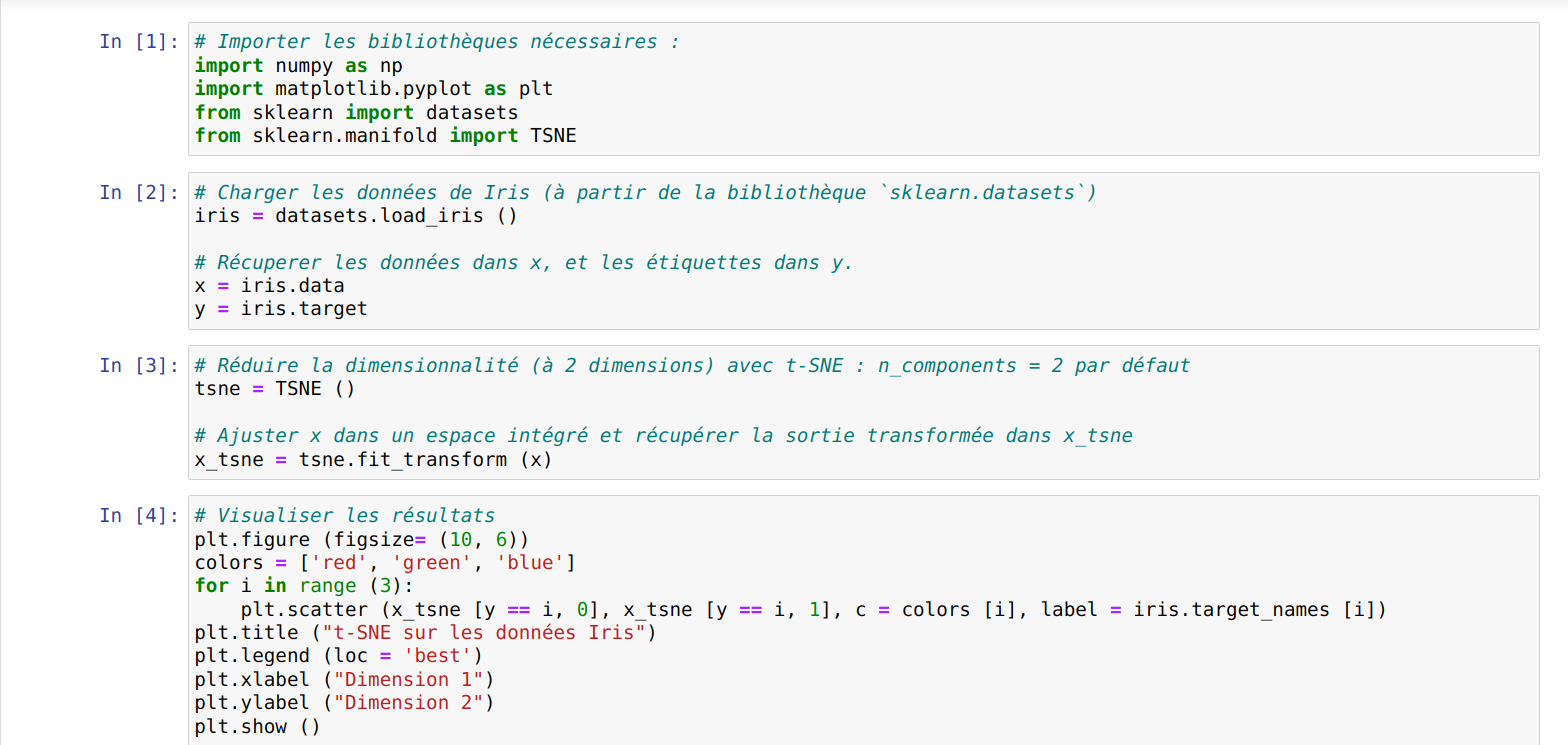
\includegraphics[width=\textwidth]{script}
		\caption{Exemple d'implémentation de t-SNE}
		\label{fig:figure1}
	\end{figure}
	
	Pour exécuter et visualiser ce scritp, veillez cliquer \href{https://github.com/hmoustaphaousmane/t-sne/blob/main/t-SNE.ipynb}{ici}.
	
	\begin{figure}[H]
		\centering
		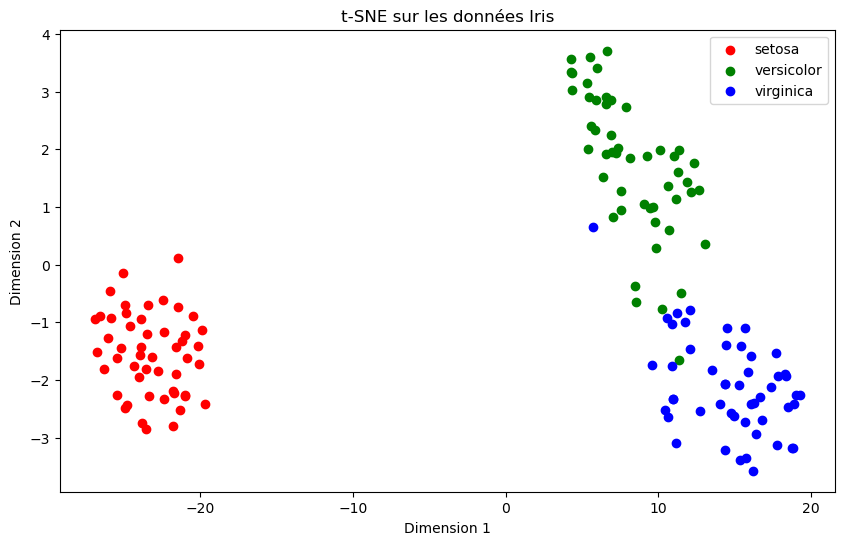
\includegraphics[width= 0.65 \textwidth]{output}
		\caption{Plot}
		\label{fig:figure2}
	\end{figure}

	\newpage
	\section*{Conclusion}
	\addcontentsline{toc}{section}{\protect\numberline{}Conclusion}
	Bref, l'algorithme t-SNE repose sur le principe de regrouper des points similaires dans l'espace d'origine pour les projeter ensuite dans un espace de dimension inférieure. Il utilise une distribution de probabilité pour mesurer la similarité entre les points dans l'espace d'origine et dans l'espace de projection. Les points similaires ont une probabilité plus élevée d'être choisis comme voisins dans l'espace de projection. Cet algorithme a des limites dont l'Analyse de la Composante Principale (ACP) apporte des solutions.
	
	\newpage
	\section*{Reférences}
	\addcontentsline{toc}{section}{\protect\numberline{}Bibliographie}
	\begin{itemize}
		\item \href{https://colab.research.google.com/drive/1wW0akEQlZ_hec1TPh8b_8HVYwXHHp1_A?usp=sharing}{Le notebook des modeules étudiés en salle}
		\item \href{https://scikit-learn.org/stable/modules/generated/sklearn.manifold.TSNE.html}{La documentation officielle de scikit-learn.}
		\item \href{https://scikit-learn.org/stable/modules/manifold.html\#t-sne}{La documentation officielle de scikit-learn (t-SNE).}
		\item \href{https://fr.wikipedia.org/wiki/Algorithme\_t-SNE}{Wikipédia}
	\end{itemize}
\end{document}